\documentclass[a4paper]{article}
\usepackage[spanish]{babel}
\usepackage[utf8]{inputenc}
\usepackage{charter}   % tipografia
\usepackage{graphicx}
\usepackage{placeins}
%\usepackage{makeidx}
%\usepackage{paralist} %itemize inline

%\usepackage{float}
%\usepackage{amsmath, amsthm, amssymb}
%\usepackage{amsfonts}
%\usepackage{sectsty}
%\usepackage{charter}
%\usepackage{wrapfig}
%\usepackage{listings}
%\lstset{language=C}


\usepackage{color} % para snipets de codigo coloreados
\usepackage{fancybox}  % para el sbox de los snipets de codigo

\definecolor{litegrey}{gray}{0.94}

% \newenvironment{sidebar}{%
% 	\begin{Sbox}\begin{minipage}{.85\textwidth}}%
% 	{\end{minipage}\end{Sbox}%
% 		\begin{center}\setlength{\fboxsep}{6pt}%
% 		\shadowbox{\TheSbox}\end{center}}
% \newenvironment{warning}{%
% 	\begin{Sbox}\begin{minipage}{.85\textwidth}\sffamily\lite\small\RaggedRight}%
% 	{\end{minipage}\end{Sbox}%
% 		\begin{center}\setlength{\fboxsep}{6pt}%
% 		\colorbox{litegrey}{\TheSbox}\end{center}}

\newenvironment{codesnippet}{%
	\begin{Sbox}\begin{minipage}{\textwidth}\sffamily\small}%
	{\end{minipage}\end{Sbox}%
		\begin{center}%
		\vspace{-0.4cm}\colorbox{litegrey}{\TheSbox}\end{center}\vspace{0.3cm}}



\usepackage{fancyhdr}
\pagestyle{fancy}

%\renewcommand{\chaptermark}[1]{\markboth{#1}{}}
\renewcommand{\sectionmark}[1]{\markright{\thesection\ - #1}}

\fancyhf{}

\fancyhead[LO]{Sección \rightmark} % \thesection\ 
\fancyfoot[LO]{\small{Alejandro Mignanelli, Facundo Barañao, Ian Sabarros}}
\fancyfoot[RO]{\thepage}
\renewcommand{\headrulewidth}{0.5pt}
\renewcommand{\footrulewidth}{0.5pt}
\setlength{\hoffset}{-0.8in}
\setlength{\textwidth}{16cm}
%\setlength{\hoffset}{-1.1cm}
%\setlength{\textwidth}{16cm}
\setlength{\headsep}{0.5cm}
\setlength{\textheight}{25cm}
\setlength{\voffset}{-0.7in}
\setlength{\headwidth}{\textwidth}
\setlength{\headheight}{13.1pt}

\renewcommand{\baselinestretch}{1.1}  % line spacing


% \setcounter{secnumdepth}{2}
\usepackage{underscore}
\usepackage{caratula}
\usepackage{url}


% ******************************************************** %
%              TEMPLATE DE INFORME ORGA2 v0.1              %
% ******************************************************** %
% ******************************************************** %
%                                                          %
% ALGUNOS PAQUETES REQUERIDOS (EN UBUNTU):                 %
% ========================================
%                                                          %
% texlive-latex-base                                       %
% texlive-latex-recommended                                %
% texlive-fonts-recommended                                %
% texlive-latex-extra?                                     %
% texlive-lang-spanish (en ubuntu 13.10)                   %
% ******************************************************** %



\begin{document}


\thispagestyle{empty}
\materia{Organización del Computador II}
\submateria{Primer Cuatrimestre de 2015}
\titulo{Trabajo Práctico II}
\subtitulo{SIMD}
\integrante{Alejandro Mignanelli}{609/11}{minga_titere@hotmail.com}
\integrante{Facundo Barañao}{480/11}{facundo_732@hotmail.com}
\integrante{Iaaaaaaan}{XXX/xx}{@gmail.com}

\maketitle
\newpage

\thispagestyle{empty}
\vfill
\begin{abstract}
En el presente trabajo se describe la problemática de procesar información de manera eficiente cuando los mismos requieren:
\begin{enumerate}
\item Transferir grandes volúmenes de datos.
\item Realizar las mismas instrucciones sobre un set de datos importante.
\end{enumerate}
\end{abstract}
\thispagestyle{empty}
\vspace{3cm}
\tableofcontents
\newpage

%\normalsize
\section{Objetivos generales}
El objetivo de este Trabajo Práctico es mostrar las variaciones en la performance que pueden ocurrir al utilizar instrucciones SIMD cuando se manejan grandes volúmenes de datos que requieren un procesamiento similar, en comparación con implementaciones que no lo utilizan.

Para ello se realizarán distintos experimentos sobre tres filtros de foto, Blur, Merge y HSL, tanto en código assembler, que aproveche las instrucciones SSE brindadas para los procesadores de arquitectura Intel, como en código C compilado con gcc, al que se le aplicará el grado de optimización grados de optimización -O3.

FALTA PONER QUE QUIERO VER PARTICULARMENTE DE CADA UNO!!!!


\newpage
\section{Preámbulo}

\subsection{Calidad de las Mediciones}
Las mediciones se realizaron corriendo los filtros 1000 veces cada uno, cuyos resultados fueron podados, eliminando 200 outliers superiores y 200 outliers inferiores. Con los restantes 600 resultados, se realizó un promedio, y estos promedios son los que se pueden apreciar en los distintos gráficos.


\newpage

\section{Experimentación}


\newpage

\section{Blur}

\subsection{Idea de las implementaciones}
A continuación se explicará un ciclo de ejecución de cada una de las implementaciones de Blur:

\subsubsection{Implementación 1}

Debido a que este filtro usa pixeles de otras posiciones de la imágen original para modificar cada pixel, consideramos pertinente contar con una copia de la imágen original, cuyo objetivo es tener un lugar seguro que no ``ensucia'' los datos de entrada de cada pixel que debo modificar. Cuando se pidió la memoria para esta copia, se le agregaron bytes de más, porque por como esta implementado, cuando se modificase el último píxel, se leería una posición de memoria que no pertenece a la imágen generando inconvenientes con VALGRIND. Esto se hace antes de un ciclo de ejecución del algoritmo, pero es importante remarcarlo. Una vez finalizado esto, dentro de un ciclo de ejecución, lo primero que hace nuestro algoritmo es cargar en tres xmm pixeles de manera tal de tener en un xmm los vecinos superiores, en otro xmm los vecinos inferiores, y en otro los vecinos del pixel a modificar, siempre tomando un pixel de más, como se muestra a continuación.
\vspace*{0.3cm}

(cada campo tiene 32 bits)

$xmm0=  basura|vecino_{sup1}|vecino_{sup2}|vecino_{sup3}$

\vspace*{0.3cm}

$xmm1=  basura|vecino_3$           $|pixel$       $|vecino_4   $

\vspace*{0.3cm}

$xmm2=  basura|vecino_{inf6}|vecino_{inf7}|vecino_{inf8}$

\vspace*{0.3cm}

Estos xmms se cargan desde la imagen copia. Como tomamos un pixel que no tiene nada que ver con el filtro, consideramos apropiado transformalo en 0. Luego desempaquetamos los tres xmm, obteniendo lo siguiente:

\vspace*{0.3cm}

(cada campo tiene 64 bits ; cada componente r,g,b,a tiene tamaño word)

\vspace*{0.3cm}
$xmm0=  0|b_{sup1}$ $g_{sup1}$ $r_{sup1}$ $a_{sup1}$ 

\vspace*{0.3cm}

$xmm1=  b_{sup2}$ $g_{sup2}$ $r_{sup2}$ $a_{sup2}|b_{sup3}$ $g_{sup3}$ $r_{sup3}$ $a_{sup3}$  

\vspace*{0.3cm}

$xmm2=  0         |b_{4}$ $g_{4}$ $r_{4}$ $a_{4}$

\vspace*{0.3cm}

$xmm3=  b_{pixel}$ $g_{pixel}$ $r_{pixel}$ $a_{pixel}     |b_{5}$ $g_{5}$ $r_{5}$ $a_{5}$

\vspace*{0.3cm}

$xmm4=  0         |b_{inf6}$ $g_{inf6}$ $r_{inf6}$ $a_{inf6} $ 

\vspace*{0.3cm}

$xmm5=  b_{inf7}$ $g_{inf7}$ $r_{inf7}$ $a_{inf7}|b_{inf8}$ $g_{inf8}$ $r_{inf8}$ $a_{inf8}$

\vspace*{0.3cm}

Luego se realiza una suma vertical entre todos los xmm, obteniendo asi un xmm que tiene en una mitad la suma de una parte de los vecinos, y en la otra mitad la suma de la otra parte de los vecinos. Desempaquetamos ese xmm resultado en dos xmm y realizamos nuevamente una suma vertical, obteniendo asi un xmm con la suma de todos los vecinos del pixel a modificar. Convertimos ese numero a float, lo dividimos por nueve (que son la cantidad de vecinos del pixel), revertimos la conversión, obteniendo int, y luego empaquetamos el resultado hasta tener el tamaño original del pixel en un sector de un xmm. Luego, utilizando la función movmaskdqu, insertamos en la imagen original el pixel modificado, y seteamos los registros para comenzar con la siguiente iteración para modificar el próximo píxel.  

\subsubsection{Implementación 2}

Esta implementación es similar a la anterior, con la excepción de que se procesarán 4 píxeles por iteración en lugar de uno. Al igual que en la implementación anterior, se copiará la imágen previamente, pidiendo bytes de más, y luego se entrará al ciclo. Dentro del ciclo, para procesar el primer pixel, se cargaran en tres xmms pixeles de manera tal de tener en un xmm los vecinos superiores, en otro xmm los vecinos inferiores, y en otro los vecinos del pixel a modificar, siempre contando con un pixel extra en cada xmm, de igual manera que en blur 1. Luego, se procesará de igual manera que en blur 1 pero en vez de empaquetar e insertar en la imágen, se guardará el resultado en un xmm. Se hará lo mismo con el procesamiento del segundo pixel. Para el píxel tres se cargarán xmm inicialmente de la misma forma, pero se hará una copia de los xmm cargados, para ser usados en el pixel 4. Se procesa el pixel 3 de igual manera que el pixel dos y uno. Para procesar el pixel cuatro, se reacomodarán las copias de los xmm cargados en el procesamiento del pixel 3, de manera tal de "simular" el hecho de que se hubieran cargado los pixels como en blur 1. Para eso, notemos que el pixel extra del procesamiento del pixel 3, es un vecino del pixel 4, y que el primer vecino de cada xmm del pixel 3, es el pixel extra del 4. Después de este reordenamiento, se procederá de igual manera que con los pixeles 1, 2 y 3.
Luego de esto, se tienen en 4 xmm los 4 píxeles procesados, se empaquetan de manera tal de tener los 4 pixeles en un xmm y se insertan en la imágen original.

\subsection{Diferencias de performance en Blur}

\begin{figure}[h]
  \centering
    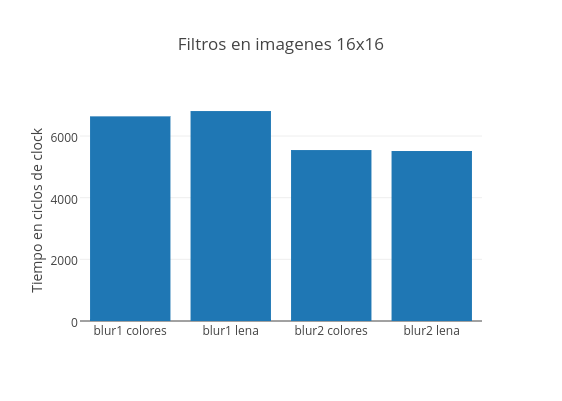
\includegraphics[width=0.75\textwidth]{imagenes/Filtros blur en imagenes 16x16.png}
  \caption{Figura 1}
  \label{fig:graficoblur1}
\end{figure}
 \FloatBarrier



\begin{figure}[h]
  \centering
    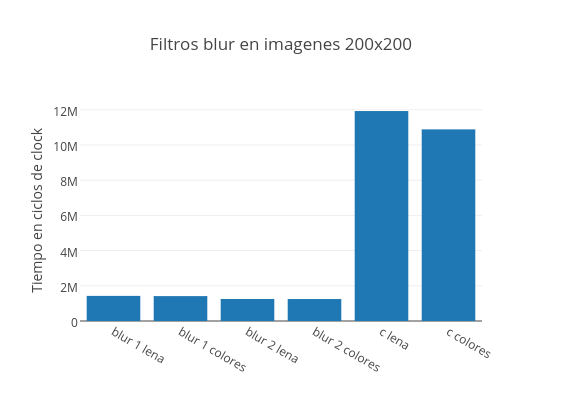
\includegraphics[width=0.75\textwidth]{imagenes/Filtros blur en imagenes 200x200.png}
  \caption{Figura 2}
  \label{fig:graficoblur2}
\end{figure}
 \FloatBarrier

\begin{figure}[h]
  \centering
    \includegraphics[width=0.75\textwidth]{imagenes/ComparacionAccesosAMemoriaBlur Colores.png}
  \caption{Figura 3}
  \label{fig:graficoblur3}
\end{figure}
 \FloatBarrier

\begin{figure}[h]
  \centering
    \includegraphics[width=0.75\textwidth]{imagenes/ComparacionConOperaciones AritmeticasBlurColores.png}
  \caption{Figura 4}
  \label{fig:graficoblur4}
\end{figure}
 \FloatBarrier


\subsubsection{Resultados}


\subsubsection{Conclusiones}


\newpage
\section{Merge}

\subsection{Idea de las implementaciones}
A continuación se explicará un ciclo de ejecución de cada una de las implementaciones de Merge (tener en cuenta que este filtro toma una imágen original, y una imágen que filtra):

\subsubsection{Implementación 1}
De las dos imágenes, tomamos 4 píxeles y los insertamos registros xmm (uno por cada imágen). A cada uno de estos, los desempaquetamos hasta obtener en 4 xmm, los cuatro pixeles de una imagen, y en otros 4 xmm los píxeles de la segunda imágen. Cada uno de los xmm anteriores, los convertimos a floats.
\vspace*{0.3cm}

(cada campo tiene 32 bits)

Imágen original:

\vspace*{0.3cm}

$xmm3 = b3_{orig} | g3_{orig} | r3_{orig} | a3_{orig}$   (cada campo es un float)

\vspace*{0.3cm}

$xmm2 = b2_{orig} | g2_{orig} | r2_{orig} | a2_{orig}$   (cada campo es un float)

\vspace*{0.3cm}

$xmm1 = b1_{orig} | g1_{orig} | r1_{orig} | a1_{orig}$   (cada campo es un float)

\vspace*{0.3cm}

$xmm0 = b0_{orig} | g0_{orig} | r0_{orig} | a0_{orig}$   (cada campo es un float)

\vspace*{0.3cm}

Imágen Filtro:

\vspace*{0.3cm}

$xmm7 = b3_{filt} | g3_{filt} | r3_{filt} | a3_{filt}$   (cada campo es un float)

\vspace*{0.3cm}

$xmm6 = b2_{filt} | g2_{filt} | r2_{filt} | a2_{filt}$   (cada campo es un float)

\vspace*{0.3cm}

$xmm5 = b1_{filt} | g1_{filt} | r1_{filt} | a1_{filt}$   (cada campo es un float)

\vspace*{0.3cm}

$xmm4 = b0_{filt} | g0_{filt} | r0_{filt} | a0_{filt}$   (cada campo es un float)

\vspace*{0.3cm}

Luego, multiplicamos los xmm correspondientes a la imágen original por value y a los xmm de la imágen filtro por 1-value. Después de esto, sumamos los xmm que representan un pixel de una imágen con su correspondiente xmm de la otra imágen y los guardamos en xmm, obteniendo 4 xmm que representan los 4 píxeles filtrados. Los convertimos nuevamente a int, y los empaquetamos de manera tal de tener en un xmm los 4 píxeles. Luego los insertamos en la imágen original.

\vspace*{0.3cm}

\subsubsection{Implementación 2}



\subsection{Diferencias de performance en Merge}

\begin{figure}[h]
  \centering
    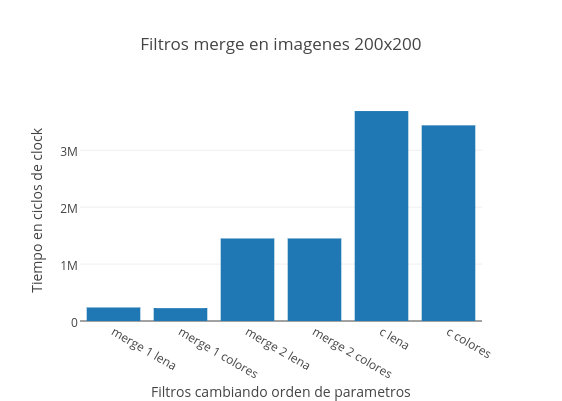
\includegraphics[width=0.75\textwidth]{imagenes/Filtros merge en imagenes 200x200.png}
  \caption{Figura 5}
  \label{fig:graficomerge1}
\end{figure}
 \FloatBarrier



\begin{figure}[h]
  \centering
    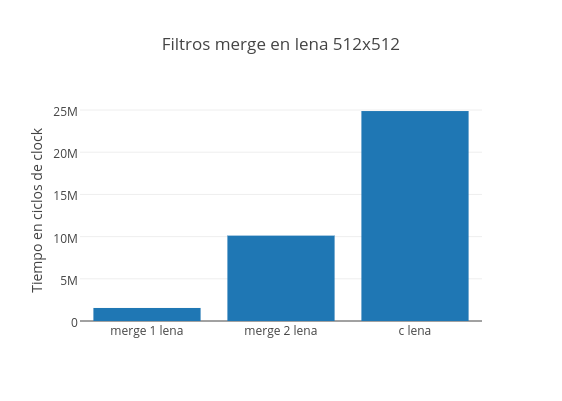
\includegraphics[width=0.75\textwidth]{imagenes/Filtros merge en lena 512x512.png}
  \caption{Figura 6}
  \label{fig:graficomerge2}
\end{figure}
 \FloatBarrier

\begin{figure}[h]
  \centering
    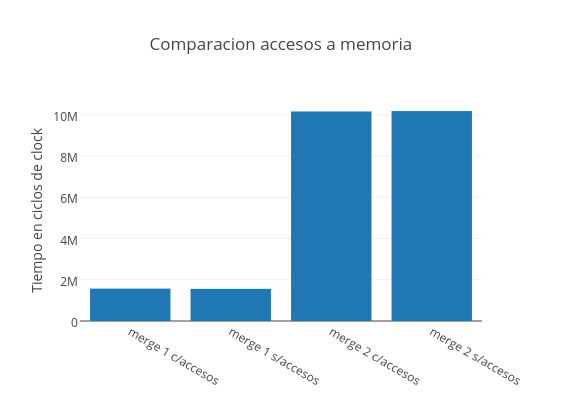
\includegraphics[width=0.75\textwidth]{imagenes/Comparacion accesos a memoria merge colores.png}
  \caption{Figura 7}
  \label{fig:graficomerge3}
\end{figure}
 \FloatBarrier

\begin{figure}[h]
  \centering
    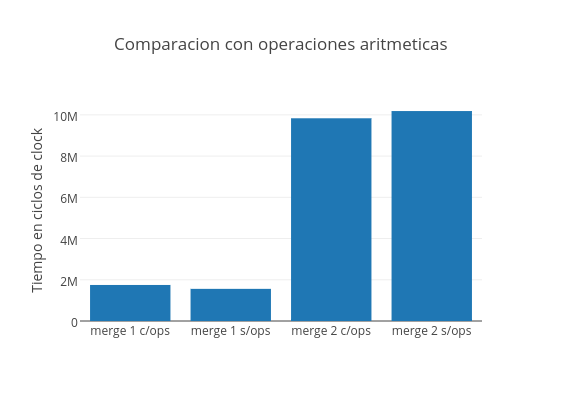
\includegraphics[width=0.75\textwidth]{imagenes/Comparacion con operaciones aritmeticas merge colores.png}
  \caption{Figura 8}
  \label{fig:graficomerge4}
\end{figure}
 \FloatBarrier



\subsubsection{Resultados}

\subsubsection{Conclusiones}


\newpage

\section{HSL}

\subsection{Idea de las implementaciones}
A continuación se explicará un ciclo de ejecución de cada una de las implementaciones de Hsl:

\subsubsection{Implementación 1}

Esta implementación usa dos funciones en c, {\tt rgbtohsl} y {\tt hsltorgb} que hacen lo que sus respectivos nombres indican, transformar un pixel en formato rgb a hsl y de hsl a rgb respectivamente. La primera precisa que se le pase como parámetro un puntero a una dirección de memoria que pueda guardar 16 bytes, donde guardará el resultado, y la segunda recibe un puntero a una dirección de memoria que tenga un hsl para convertir en rgb e introducir en la imágen. Para esto, antes de entrar a un ciclo, se pide por malloc 16 bytes, cuyo puntero se guardara en un registro (a fines prácticos, r8).
Otros aspectos a destacar antes de empezar a explicar la implementación de un ciclo, es que los valores HH, SS y LL se encuentran en tres xmm distintos de la siguiente manera:

\vspace*{0.3cm}

(cada campo tiene 32 bits)

\vspace*{0.3cm}

$xmm3=0|0|HH|0$

\vspace*{0.3cm} 

$xmm1=0|SS|0|0$

\vspace*{0.3cm}

$xmm2=LL|0|0|0$

\vspace*{0.3cm}

Inicio mi ciclo de ejecución pasándole el píxel a la función {\tt rgbtohsl}, obteniendo así en r8 un puntero al hsl del píxel. Luego paso el hsl a un xmm (digamosle xmm0), para poder trabajar con él, y a este le sumo los xmm que representan HH, SS y LL, obteniendo lo siguiente.

(cada campo representa 32bits)

\vspace*{0.3cm}

$xmm0=l+LL|s+SS|h+HH|a$

\vspace*{0.3cm}

Este xmm, lo copio en otros dos xmm, uno al cual le aplico la función {\tt roundps} junto con la opción de redondeo hacia abajo, y luego le aplico {\tt cvtps2dq}, y al otro {\tt cvttps2dq}. De esta manera, en el xmm original voy a guardar el resultado (este mantiene su tipo float), y los otros dos los uso para hacer comparaciones (de habernos dado cuenta antes de la instruccion cmpps, se podría haber evitado esto). Llamemos estas dos copias xmm4 (la de roundps+cvt) y xmm5(la de cvtt).Luego de estas preparaciones vamos al corazón del ciclo.

\paragraph*{Cálculo de H:}

Muevo xmm5 a otros dos xmm, a estos los comparo con una máscara que tiene un 360 (en int) en la posición de h, y un 0 en el resto, siendo cada campo un doubleword. A uno de ellos lo comparo por igual, al otro por mayor, y a ambos les dejo en 0 todos los campos salvo el correspondiente a h. Muevo lo que hay en xmm4 a otros dos xmm y les aplico lo mismo que les aplique a las copias de xmm5, con la diferencia de que la máscara utilizada en este caso tiene un 0 (en int) en el lugar de h en vez de un 360 y el resto de los campos estan cubiertos por 1s. Luego de estas operaciones, se obtendría lo siguiente:

\vspace*{0.3cm}

(cada campo tiene 32 bits, si la pregunta se responde por afirmativo, entonces todos los bits del campo serán 1s, caso contrario, serán 0s)

\vspace*{0.3cm}

Copias de xmm5:

\vspace*{0.3cm}

$xmm8= 0 | 0 | h+hh = 360? | 0$

\vspace*{0.3cm} 

$xmm9=0 | 0 | h+hh > 360? | 0$

\vspace*{0.3cm}

Copias de xmm4:

\vspace*{0.3cm}

$xmm10= 0 | 0 | h+hh = 0? | 0$

\vspace*{0.3cm}

$xmm11= 0 | 0 | h+hh > 0? | 0$

\vspace*{0.3cm}

Veamos que como xmm5 está convertido a int por truncamiento, efectivamente sirve para comparar si es mayor o igual a 360, puesto que si el número es menor, nunca redondea para arriba. Si bien es cierto que a un número como 360.4 lo transforma en 360, nos interesa poder decir si el número es mayor o igual, y no nos interesa por cual de los dos casos entre. Por otro lado, veamos que no sirve para comparar si es mayor o igual a 0, puesto que si el número fuera por ejemplo -0.4, el truncamiento lo transforma en 0, y obtengo una respuesta afirmativa, cuando debería ser negativa. Por eso para esto usamos las copias de xmm4, ya que al tomarlas por redondeo hacia abajo darán -1. Nuevamente, nos interesa el mayor o igual, y no en cual caso cayó específicamente, por lo cual el hecho de convertir números como 0.99 a 0 no tendrá relevancia.

LLegado este punto, realizaremos un {\tt pxor} entre las copias de xmm5 para saber si el h+HH es mayor o igual a 360 (supongamos que dejamos esto en xmm8), y otro {\tt pxor} entre las copias de xmm4 para saber si el h+HH es mayor o igual a 0. A las copias de xmm4 las negaremos para saber ahora si h+HH es menor a 0(supongamos que dejamos esto en xmm10). Luego a estos dos registros le pasaremos la máscara utilizada para las copias de xmm5 (la que tiene un 360 en h), obteniendo lo siguiente:

\vspace*{0.3cm}

(cada campo tiene 32 bits)

\vspace*{0.3cm}

$xmm8= 0 | 0 | 360$ $si$ $h+hh>=360,$ $0$ $sino$ $| 0$

\vspace*{0.3cm}

$xmm10=0 | 0 | 360$ $si$ $h+hh<360,$ $0$ $sino$ $| 0$

\vspace*{0.3cm}

Ahora veamos lo siguiente. Como un número no puede ser mayor o igual a 360 y menor que 0 a la vez, solo uno de ellos tendra un 360, y el otro tendrá 0. Entonces, convertimos estos xmm a floats, tomamos el xmm original, el que llamamos xmm0, le sumamos verticalmente xmm8, y le restamos xmm10, obteniendo asi el h+HH correspondiente según el filtro suma de hsl.

\paragraph*{Cálculo de S y L:}

Son exactamente iguales entre si, teniendo en cuenta que su posición en el xmm es diferente, y muy parecidos al cálculo de h+HH hasta cierto punto, salvo por las siguientes diferencias:

\begin{itemize}
	\item Se usa una máscara que tiene un 1 en l o s dependiendo el caso, en vez de la mascara que tiene un 360 en h.
	\item Se compara si los s+SS y l+LL son mayores iguales a 1, o mayores iguales a 0.
\end{itemize}

El punto en que empiezan a diferir es luego de llegar al siguiente checkpoint (como ya explicamos, los calculos sobre s y l son bastante similares):

\vspace*{0.3cm}

(cada campo tiene 32 bits, si la pregunta se responde por afirmativo, entonces todos los bits del campo seran 1s, caso contrario, serán 0s)

\vspace*{0.3cm}

Copias de xmm5:

\vspace*{0.3cm}

$xmm8= 0 | s+SS = 1?| 0 | 0$

\vspace*{0.3cm} 

$xmm9=0 |s+SS > 1?| 0 | 0$

\vspace*{0.3cm}

Copias de xmm4:

\vspace*{0.3cm}

$xmm10= 0 |s+SS= 0?| 0 | 0$

\vspace*{0.3cm}

$xmm11= 0 |s+SS > 0?| 0 | 0$

\vspace*{0.3cm}

Luego de esto, para calcular s, realizaremos un {\tt pxor} entre las copias de xmm5 para saber si el s+SS es mayor o igual a 1 (supongamos que dejamos esto en xmm8), y otro {\tt pxor} entre las copias de xmm4 para saber si el s+SS es mayor o igual a 0 (supongamos que esto esta en xmm10).

Luego, con ayuda de los xmm antes mencionados, chequeamos si s+SS es mayor o igual a 1, y de serlo le colocamos un 1.0 en el campo de s. De no ser mayor o igual a 1, pero ser mayor igual a 0, colocamos s+SS en el campo de s, y en otro caso, lo dejamos en 0, obteniendo la parte de s correspondiente con el filtro de hsl aplicado. 

Al terminar las tres partes del filtro, y tenerlas en un xmm, copiamos el contenido de este en el puntero antes pedido, y llamamos a hsltorgb, quien coloca el pixel en la imágen.

\subsubsection{Implementación 2}
La segunda implementación es igual a la primera, salvo porque no contamos con las funciones hsltorgb y rgbtohsl, razón por la cual no se pidió memoria. En cambio, nosotros tuvimos que crear estas funciones en assembler. La explicación de un ciclo de ejecución se puede dividir en cuatro partes: La función principal, la funcion {\tt rgbtohsl\_asm}, la función {\tt hsltorgb\_asm} y la función {\tt hago\_suma}. Se explicarán primero las funciones que están contenidas en la función principal para mayor entendimiento

\paragraph*{rgbtohsl_asm:}

A la función le entran 4 píxeles por un xmm, a los cuales primero los broadcastea de manera tal de dejar en cuatro campos de 32bits todos los r juntos, todos los g juntos, todos los b juntos y todos los a juntos. Luego, desempaquetamos el xmm hasta obtener cuatro xmms de manera tal que uno tenga todos los r, otro todos los g, etc. Luego de esto los xmma quedarían con esta forma:

\vspace*{0.3cm}

(cada campo tiene 32 bits)

\vspace*{0.3cm}

 $xmm1$ $=$ $r3|r2|r1|r0$

\vspace*{0.3cm}

 $xmm2$ $=$ $g3|g2|g1|g0$

\vspace*{0.3cm}

 $xmm3$ $=$ $b3|b2|b1|b0$

\vspace*{0.3cm}

 $xmm4$ $=$ $a3|a2|a1|a0$

\vspace*{0.3cm}

Cálculo los máximos entre r,g y b de cada píxel, y los dejo en un xmm. Hago lo mismo con los mínimos, y los pongo en otro xmm. Calculo la resta entre los máximos y los mínimos y los pongo en otro xmm (a esta resta para fines prácticos la llamaremos d). Obtendríamos lo siguiente:

 \vspace*{0.3cm}

(cada campo tiene 32 bits)

\vspace*{0.3cm}

 $xmm5$ $=$ $max(r3,g3,b3)|max(r2,g2,b2)|max(r1,g1,b1)|max(r0,g0,b0)$

\vspace*{0.3cm}

 $xmm6$ $=$ $min(r3,g3,b3)|min(r2,g2,b2)|min(r1,g1,b1)|min(r0,g0,b0)$

\vspace*{0.3cm}

 $xmm7$ $=$ $max(r3,g3,b3)-min(r3,g3,b3)|max(r2,g2,b2)-min(r2,g2,b2)|$
 
 \hspace*{1.45cm}$max(r1,g1,b1)-min(r1,g1,b1)|max(r0,g0,b0)-min(r0,g0,b0)$

\vspace*{0.3cm}


Luego de estos preparativos, la función se divide en tres partes:

\begin{enumerate}
	\item Cálculo de L:
	
	Básicamente sumo verticalmente los xmm que tienen los máximos y los mínimos, los convierto en float y los divido por 510. Esto lo guardo en un xmm. Este xmm tiene los L de los 4 píxeles.
	
	\item Cálculo de S:	
	
Tomo el xmm resultado del cálculo de L, y lo copio en otro xmm. A esta copia la multiplico por dos en cada campo, y luego le resto 1.0 a cada campo. Para calcular el fabs comparo por máximo a este xmm, y a otro xmm que sea el resultado de un xmm lleno de ceros restado verticalmente con el primer xmm. La idea detrás de esto es que, sea $e$ un numero entero, entonces $fabs(e) = e$ o $-e$. Hasta ahora, me quedaría algo como:

\vspace*{0.3cm}

(cada campo tiene 32 bits)

\vspace*{0.3cm}
	
$xmm7$ $=$ $fabs(2*L3 - 1) |fabs(2*L2 - 1)|fabs(2*L1 - 1)| fabs( 2*L0 - 1)$	
	
\vspace*{0.3cm}

Después a un xmm que tenga un 1.0 por campo con campos de 32 bits, le resto el resultado anterior y lo guardo en un xmm. Tomo el xmm que tenía los máximos - mínimos, los convierto a floats, y los divido por el xmm que me guarde anteriormente. A este resultado lo divido por un xmm que tenga en los cuatro campos el número 255.0001. Luego de esto, se obtendría lo siguiente:  

\vspace*{0.3cm}

(cada campo tiene 32 bits)

\vspace*{0.3cm}

$xmm9 -> d3 / (1 - fabs(2*L3 - 1)) / 255.0001$ $|$ $d2 / (1 - fabs(2*L2 - 1)) / 255.0001$ $|$

\hspace*{1.75cm}$d1 / (1 - fabs(2*L1 - 1)) / 255.0001$ $|$ $ d0/ (1 - fabs( 2*L0 - 1)) / 255.0001$

\vspace*{0.3cm}
	
Luego compararé los máximos con los mínimos, y a aquellos que sean iguales, se les asignará un 0. En caso contrario se asignará el resultado anterior. Asi se encontraran los s para cada píxel.

	\item Cálculo de h:

	Tomo los xmm que tenían los r, g y b de los distintos píxeles, y los conviero a floats. Luego dejo en otros 3 xmm las restas de los r con los g, los g con los b, y los b con los r. Como ahora tengo que dividirlo por los $d$, pero este valor podría ser cero, teniendo en cuenta que si no es 0 es positivo, hacemos lo siguiente. Tomamos a los d, les resto uno, tomo su valor absoluto y le sumo 1. Si d era un valor positivo, debería obtener el mismo número. Caso contrario, o sea, si d era 0, debo obtener el número 2, que me va a servir solo para no dividir por cero. Haciendole esta modificación al d, los transformo a float, y ahora tomo a cada uno de los 3 xmms antes mencionados (las restas) y los divido por d. Hasta acá el estado de los xmm debería ser el siguiente:
	
\vspace*{0.3cm}

(cada campo tiene 32 bits)	
	
\vspace*{0.3cm}	

$xmm12=(r3-g3)/d3$ $|$ $(r2-g2)/d2$ $|$ $(r1-g1)/d1$ $|$ $(r0-g0)/d0$

\vspace*{0.3cm} 
 
$xmm13=(g3-b3)/d3$ $|$ $(g2-b2)/d2$ $|$ $(g1-b1)/d1$ $|$ $(g0-b0)/d0$

\vspace*{0.3cm}

$xmm14=(b3-r3)/d3$ $|$ $(b2-r2)/d2$ $|$ $(b1-r1)/d1$ $|$ $(b0-r0)/d0$	
	
\vspace*{0.3cm}
	
	Luego, a lo que recién en el estado de los xmm llamé xmm14, debo sumarle 2, al que llamamos xmm12 hay que sumarle 4, y al que llame xmm13, hay que sumarle 6. Luego, a estos 3 hay que multiplicarlos por 60. El nuevo estado debería ser el siguiente:
	
\vspace*{0.3cm}

(cada campo tiene 32 bits)	
	
\vspace*{0.3cm}	

$xmm12=60*(((r3-g3)/d3)+2)$ $|$ $60*(((r2-g2)/d2)+2)$ $|$ $60*(((r1-g1)/d1)+2)$ $|$ $60*(((r0-g0)/d0)+2)$

\vspace*{0.3cm} 
 
$xmm13=60*(((g3-b3)/d3)+2)$ $|$ $60*(((g2-b2)/d2)+2)$ $|$ $60*(((g1-b1)/d1)+2)$ $|$ $60*(((g0-b0)/d0)+2)$

\vspace*{0.3cm}

$xmm14=60*(((b3-r3)/d3)+2)$ $|$ $60*(((b2-r2)/d2)+2)$ $|$ $60*(((b1-r1)/d1)+2)$ $|$ $60*(((b0-r0)/d0)+2)$	
	
\vspace*{0.3cm}
	 
	 Ahora moveremos información a un xmm de la siguiente manera: si los máximos y los mínimos de dos campos son iguales, entonces en ese campo habrá un 0. Si el máximo de un campo es igual al r del píxel correspondiente, entonces el campo tendrá a su correspondiente en xmm13. De no ser el máximo del campo igual al r del píxel, pero si a g, entonces el campo tendrá a su correspondiente en xmm14. de no ser el máximo del campo igual al r ni al g del píxel, entonces será igual a b, y tendrá a su correspondiente en xmm12. Luego, por medio de comparaciones se observa si este xmm obtenido es mayor o igual a 360, y en caso de serlo se le resta 360.
	
\end{enumerate}

Una vez terminado esto tenemos en 3s xmm distintos los h los s y los l de cada pixel, de la siguiente manera:

\vspace*{0.3cm}

(cada campo tiene 32 bits)	
	
\vspace*{0.3cm}	

$xmm1 = H3|H2|H1|H0$

\vspace*{0.3cm}

$xmm2 = S3|S2|S1|S0$

\vspace*{0.3cm}

$xmm3 = L3|L2|L1|L0$

\vspace*{0.3cm}

$xmm4 = A3|A2|A1|A0$

\vspace*{0.3cm}

Luego, tan sólo se acomoda la información usando {\tt blendps}, {\tt shuffles} y {\tt shifts}, hasta obtener lo siguiente:

 \vspace*{0.3cm}

(cada campo tiene 32 bits)	
	
\vspace*{0.3cm}	

$xmm1 = L3|S3|H3|A3$

\vspace*{0.3cm}

$xmm2 = L2|S2|H2|A2$

\vspace*{0.3cm}

$xmm3 = L1|S1|H1|A1$

\vspace*{0.3cm}

$xmm4 = L0|S0|H0|A0$

\vspace*{0.3cm}

y esto devuelve la función.

\paragraph{hago_suma:}

Es exactamente lo explicado en la implementación uno.


\paragraph*{hsltorgb_asm:}

Esta función toma un hsl y lo transforma en un rgb. Su explicación se divide en varias partes:

\begin{enumerate}
	\item Cálculo de c:
	Copiamos el hsl a otro xmm, duplicamos todos sus campos y les restamos 1.0. Luego, usamos el truco anteriormente explicado para aplicar fabs, y ubicaremos la resta entre 1.0 y este número en un xmm. Hasta el momento, este xmm debería ser algo así:
	
\vspace*{0.3cm}

(cada campo tiene 32 bits)	
	
\vspace*{0.3cm}	
	
	$xmm4 = 1-fabs(2*l - 1)|irrelevante|irrelevante|irrelevante$
		
\vspace*{0.3cm}

Luego, copio nuevamente el xmm que tiene el hsl en otro xmm, y con un shifteo posiciono la s en el campo de la parte más alta del registro. Luego de hacer esto, multiplico el registro que shiftie con el que realice operaciones anteriormente, obteniendo asi:

\vspace*{0.3cm}

(cada campo tiene 32 bits)	
	
\vspace*{0.3cm}	
	
	$xmm4 = s*(1-abs(2*l - 1))=c|irrelevante|irrelevante|irrelevante$
		
\vspace*{0.3cm}
		
	Y con un simple broadcasteo, consigo que en todos los campos del xmm se encuentre c.
	
	\item Cálculo de x:		
		
Tomo el xmm que tiene hsl y lo copio a otro registro(el campo que nos interesará es el de h). A este lo divido por 60 y me preparo para realizar el fmod. Demonos cuenta que $fmod(x,y) = x-redondeohaciaabajo(x/y) * y$. Por esto, guardaremos en otro xmm el resultado anterior, luego en esa copia dividiremos todos los campos por dos, redondearemos hacia abajo, multiplicar los campos por 2, y luego al resultado original lo restaremos con este, obteniendo el fmod. Por el momento los xmm deberían quedar de la siguiente manera:

\vspace*{0.3cm}

(cada campo tiene 32 bits)	
	
\vspace*{0.3cm}	

$xmm1 -> irrelevante|irrelevante|fmod(h/60.0 , 2)|irrelevante$ 		
		
\vspace*{0.3cm}		
		
	A este xmm le resto uno en cada campo y le calculo fabs como comentamos anteriormente. Luego tomo un xmm que tenga un 1.0 en cada campo, y le resto el resultado anterior. A esto lo multiplico por la c obtenida anteriormente, teniendo como resultado lo siguiente:
	
\vspace*{0.3cm}

(cada campo tiene 32 bits)	
	
\vspace*{0.3cm}	

	$xmm1 -> irrelevante|irrelevante|c*(1-fabs(fmod(h/60.0 , 2) -1))=x|irrelevante$
		
\vspace*{0.3cm}
	
Luego, broadcasteo de manera tal que tenga x en todos los campos.	
	
	\item Cálculo de m:
	
Tomo el c antes obtenido, lo copio en un xmm, a esta copia la divido por 2, y luego copio otro xmm el hsl de entrada, a cuya copia le restare el resultado anterior. Como resultado de estas operaciones, obtendremos el siguiente xmm:

$xmm3 -> L-(c/2)=m | c/2 | c/2 | c/2$
	
	Luego usando shuffle barajo los campos para obtener una m en cada uno de ellos.
	
	\item Cálculo de RGB:
	
		
	
\end{enumerate}

\subsection{Diferencias de performance en HSL}

\begin{figure}[h]
  \centering
    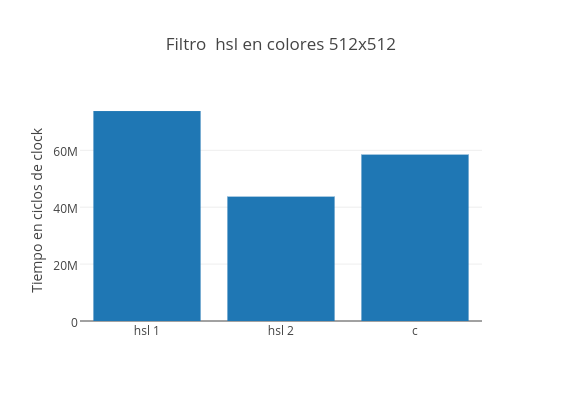
\includegraphics[width=0.75\textwidth]{imagenes/FiltroHslEnColores512x512.png}
  \caption{Figura 7}
  \label{fig:graficohsl1}
\end{figure}
 \FloatBarrier

\begin{figure}[h]
  \centering
    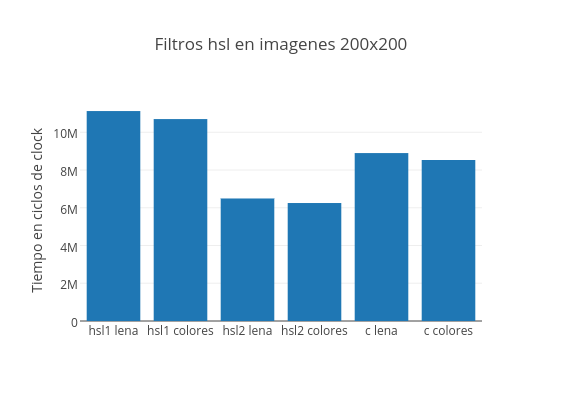
\includegraphics[width=0.75\textwidth]{imagenes/Filtros hsl en imagenes 200x200.png}
  \caption{Figura 8}
  \label{fig:graficohsl2}
\end{figure}
 \FloatBarrier

\begin{figure}[h]
  \centering
    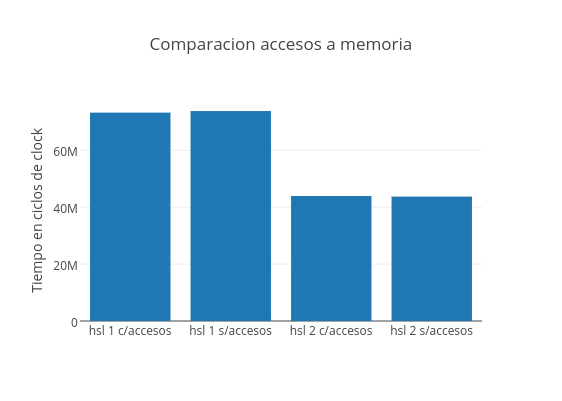
\includegraphics[width=0.75\textwidth]{imagenes/Comparacion accesos a memoria hsl colores.png}
  \caption{Figura 9}
  \label{fig:graficohsl3}
\end{figure}
 \FloatBarrier

\begin{figure}[h]
  \centering
    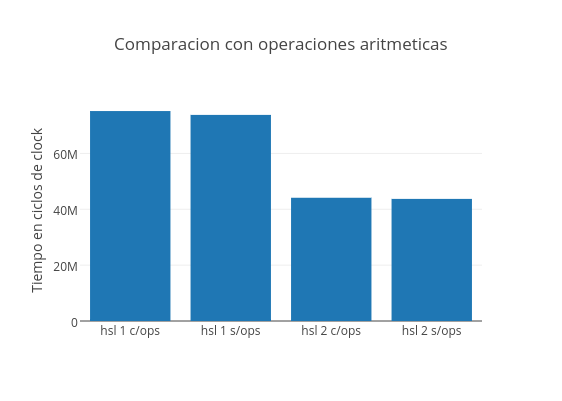
\includegraphics[width=0.75\textwidth]{imagenes/Comparacion con operaciones aritmeticas hsl colores.png}
  \caption{Figura 10}
  \label{fig:graficohsl4}
\end{figure}
 \FloatBarrier

\begin{figure}[h]
  \centering
    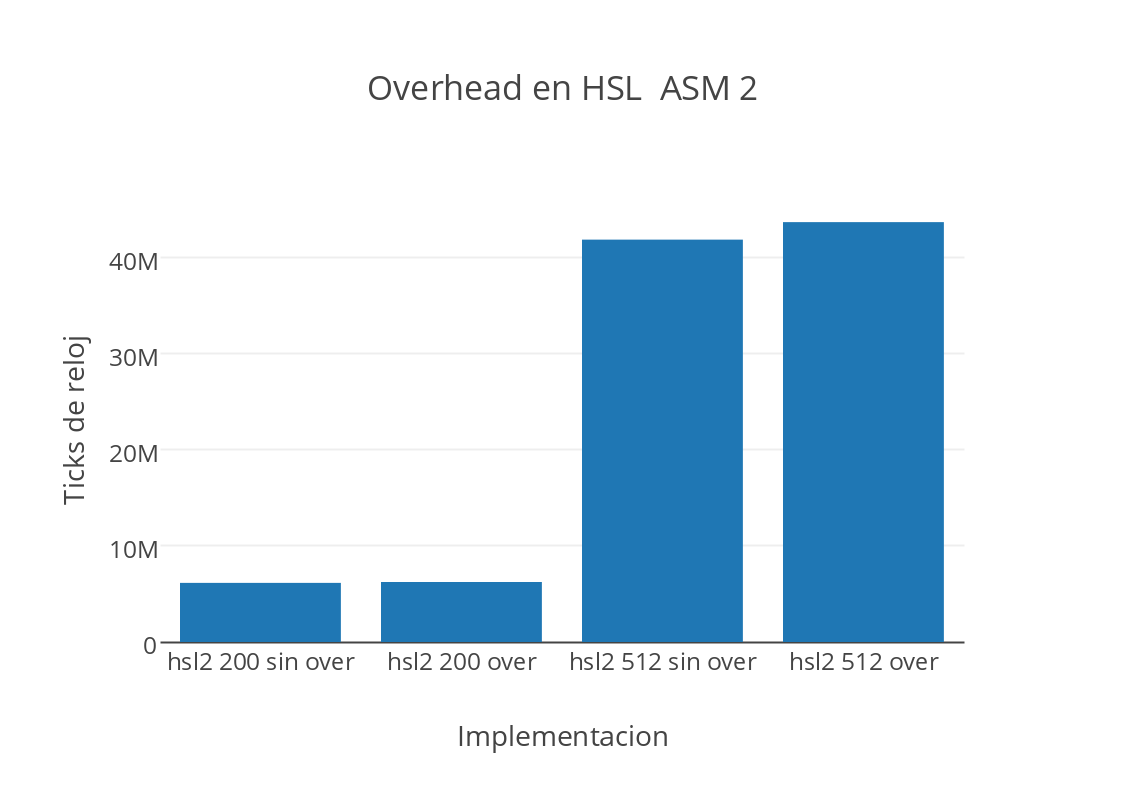
\includegraphics[width=0.75\textwidth]{imagenes/OverheadEnHSLASM2}
  \caption{Figura 11}
  \label{fig:Overheadhsl}
\end{figure}
 \FloatBarrier

\subsubsection{Resultados}

\subsubsection{Conclusiones}


\newpage
\section{Conclusiones y trabajo futuro}


\end{document}

